
\section{Задание 3. ДУ второго порядка}

\textbf{Условие.}

Пружинный маятник движется по закону:

\[y^{\prime\prime} + p(t)y^\prime + q(t)y = f(t)\]

\begin{enumerate}
    \item Запишите однородное уравнение движения маятника. Выясните, почему движение описывается уравнением такого вида (каков физический смысл коэффициентов левой части уравнения).
    \item Установите характер движения (периодический, апериодический) при данных $p(t)$ и $q(t)$.
    \item Найдите ФСР ЛОДУ и убедитесь в ее линейной независимости с помощью вронскиана.
    \item Найдите общее решение ЛОДУ.
    \item Задайте начальные условия в момент $t_0 = 0$ и найдите удовлетворяющее им частное решение ЛОДУ. Изобразите закон движения в системе координат.
    \item Составьте линейное неоднородное дифференциальное уравнение (ЛНДУ) с правой частью $f(t)$. Выясните физический смысл функции $f(t)$.
    \item Найдите решение ЛНДУ, удовлетворяющее начальным условиям. Изобразите закон движения в системе координат.
    \item Сделайте вывод о влиянии на движение функции $f(t)$.
\end{enumerate}

\[p(t) = 4, q(t) = 5, f(t) = t^2 e^{2t}\]

\vspace{10mm}
\textbf{Решение.}

\begin{enumerate}
    \item $y^{\prime\prime} + 4y^\prime + 5y = 0$ \\
        Формула колебаний пружинного маятника с затуханием: \\
        $y^{\prime\prime} + \frac{c}{m}y^\prime + \frac{k}{m}y = f(t)$ \\
        Где $m$ - масса груза, $k$ - коэффициент упругости и $c$ - коэффициент затухания от скорости. \\
        Значит в идеальной системе $y^{\prime\prime} + q(t)y = t^2 e^{2t}$, ускорение зависит от координаты. \\
        В нашем случае с затуханием система должна будет стабилизироваться в нуле энергии (без движении). \\
    \item $y^{\prime\prime} + 4y^\prime + 5y = 0$ \\
        $\lambda^2 + 4\lambda + 5 = 0$ \\
        $\lambda = \pm i - 2$ \\
        $y(t) = \frac{C_1 \cos(t)}{e^{2t}} + \frac{C_2 \sin(t)}{e^{2t}}$ \\
        Движение периодическое. \\
    \item $y(t) = \frac{C_1 \cos(t)}{e^{2t}} + \frac{C_2 \sin(t)}{e^{2t}}$ \\
        ФСР: $\{\frac{\cos(t)}{e^{2t}}, \frac{\sin(t)}{e^{2t}}\}$ \\
        $W = \begin{vmatrix}
            \frac{\cos(t)}{e^{2t}} & \frac{\sin(t)}{e^{2t}} \\
            -\frac{e^{2t}\sin(t) + 2e^{2t}\cos(t)}{e^{4t}} & \frac{e^{2t}\cos(t) - 2e^{2t}\sin(t)}{e^{4t}}
        \end{vmatrix} = \frac{e^{2t}\cos^2(t) - e^{2t}\sin(2t)}{e^{6t}} + \frac{e^{2t}\sin^2(t) + e^{2t}\sin(2t)}{e^{6t}} = \frac{e^{2t}}{e^{6t}} = e^{-4t}$ \\
        $W \neq 0$ $\Longrightarrow$ система линейно независима по теореме Коши. \\
    \item Общее решение: $y(t) = \frac{C_1 \cos(t)}{e^{2t}} + \frac{C_2 \sin(t)}{e^{2t}}$ \\
    \item Пусть $y(t_0) = 1$, $y^\prime(t_0) = 0$

        $
        \begin{cases}
            y(t_0) = \frac{C_1 \cos(t)}{e^{2t}} + \frac{C_2 \sin(t)}{e^{2t}} \\
            y^\prime(t_0) = -\frac{C_1 (e^{2t}\sin(t) + 2e^{2t}\cos (t)) }{e^{2t}} + \frac{C_2 ( e^{2t} \cos(t) - 2e^{2t} \sin(t))}{e^{2t}}
        \end{cases}
        \begin{cases}
            1 = C_1 \\
            0 = C_2 - 2 C_1
        \end{cases}
        \begin{cases}
            1 = C_1 \\
            2 = C_2
        \end{cases}
        $

        	Частное решение ЛОДУ: $y = \frac{\cos(t)}{e^{2t}} + \frac{2\sin(t)}{e^{2t}}$ 

	\begin{center}
	        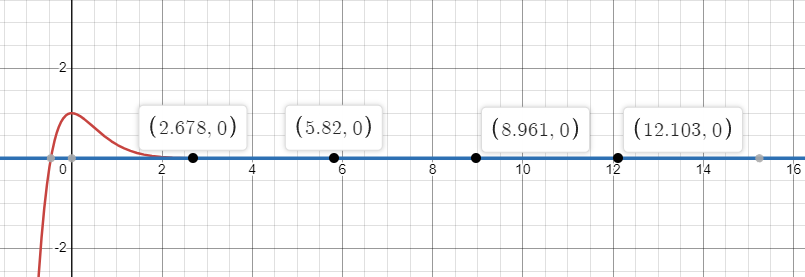
\includegraphics[height=60mm]{images/3_5}
	\end{center}	

	Из точек пересечения с осью абсцисс видим переодичность движения.

    \item $y^{\prime\prime} + 4y^\prime + 5y = t^2 e^{2t}$ \\
        $f(t)$ (в нашем случае $t^2 e^{2t}$) - действие внешних сил на систему. \\
    \item $W_1 = \begin{vmatrix}
            0 & \frac{\sin(t)}{e^{2t}} \\
            t^2e^{2t} & \frac{e^{2t}\cos(t) - 2e^{2t}\sin(t)}{e^{4t}}
        \end{vmatrix} = -t^2 e^{2t} \cdot \frac{\sin(t)}{e^{2t}} = -t^2 \cdot \sin(t)$\\
        $W_2 = W = \begin{vmatrix}
            \frac{\cos(t)}{e^{2t}} & 0 \\
            -\frac{e^{2t}\sin(t) + 2e^{2t}\cos(t)}{e^{4t}} & t^2e^{2t}
        \end{vmatrix} = \frac{\cos(t)}{e^{2t}} \cdot t^2 e^{2t} = \cos(t) \cdot t^2$\\
        $C_1^\prime(t) = \frac{W_1}{W} = -t^2\sin(t)e^{4t}$ \\
        $C_2^\prime(t) = \frac{W_2}{W} = t^2\cos(t)e^{4t}$ 

        $C_1(t) = \int -t^2\sin(t)e^{4t}\ dt = \frac{e^{4 t} ((94 - 272 t + 289 t^2) \cos(t) - 2 (52 - 255 t + 578 t^2) \sin(t))}{4913}$

        $C_2(t) = \int t^2\cos(t)e^{4t}\ dt =\frac{e^{4 t} (2 (52 - 255 t + 578 t^2) \cos(t) + (94 - 272 t + 289 t^2) \sin(t)))}{4913}$

	Общее решение ЛНДУ: $y(t) = \frac{C_1\cos(t)}{e^{2t}} + \frac{C_2\sin(t)}{e^{2t}} + \frac{1}{17}e^{2t}t^2 - \frac{16}{289}e^{2t}t + \frac{94}{4913}e^{2t}$. 

Частное решение ЛНДУ: $y(t) = \frac{4819}{4913} \frac{\cos(t)}{e^{2t}} + \frac{9722}{4913} \frac{\sin(t)}{e^{2t}} + \frac{1}{17}e^{2t}t^2 - \frac{16}{289}e^{2t}t + \frac{94}{4913}e^{2t}$

	\begin{center}
	        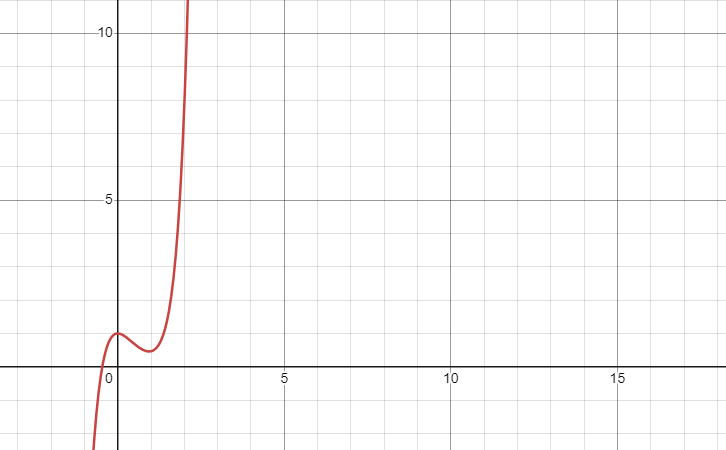
\includegraphics[height=60mm]{images/3_7}
	\end{center}	

    \item Внешняя сила $f(t)$ слишком сильно действует на маятник, так что он не будет колебаться, а будет крутиться.


\end{enumerate}




